\section{Resultados}\label{results}
%All results presented in this section are relative to the application layer. We run simulations on a computer with 2GB RAM memory, CPU intel dual core i3, and Ubuntu 18.04.1 LTS operating system. All runs last 101 seconds with the first second used just for network setup (e.g., nodes requesting connections). The simulation was executed 20 times with $95\%$ of confidence interval.
%Using some \textit{api} from Castalia Simulator some results like the total number of control packets exchanged, the total number of measurements packets, how many times a packets was retransmited among many others results can be obtained easily.
Todos os resultados apresentados nesta seção são relativos à camada de aplicação implementada por este trabalho. As simulações foram feitas em um computador com 8GB de mémoria RAM, Intel Core i5-7200U e sistema operacional Ubuntu 18.04.1 LTS. A simulação tem duração de $101s$, sendo o primeiro segundo apenas para a configuração da camada MAC. Foram executadas $15$ repetições da simulação com intervalo de confiança de $95\%$. 
%Devido à escala de alguns gráficos, nem sempre o intervalo de confiança fica muito visível. 

\subsection{Casos de Uso e Parâmetros da Simulação}

%Remote Monitoring and Independent living for elderly care is one of the use cases of the X73-PHD standard. The sensors and actuators proposed for this use case are: blood pressure, thermometer, glucose meter, pulse oximeter and basic ECG  \cite{b3}. In this work, we have used an hypothetical elderly patient who has cardiac problems, diabetes and hypertension, and needs to be monitored in his home.
Monitoramento remoto de pacientes e independência para a terceira idade são casos de uso discutidos no padrão X73-PHD. Os sensores e atuadores propostos para esses dois casos de usos são: medidor de pressão, termômetro, medidor de glicose, oxímetro de pulso e um eletrocardiograma.

%Figure~\ref{fig:wbantopology} shows the topology setup used in our simulation. The hub node is placed at the right hip, a sensor node at each wrist, one sensor node at the each ankle, and one sensor on the chest. We used this set to test our proposed features. These nodes' positions have the advantage of experimental measurements of path loss, made for every pair of nodes, as discussed in \cite{b4}.
A Figura \ref{fig:wbantopology} mostra a topologia utilizada nas simulações. O hub, que é o nó gerente, está localizado no quadril direito, um nó sensor em cada pulso e um em cada tornozelo e um sensor no meio do peito. Utilizando essas posições, temos a vantagem de utilizar um canal sem fio que já possui um modelo de perda de sinal, entre cada par de dispositivos, pré-definido com experimentos reais, conforme apresentado em \cite{b4}.

%\begin{figure}[htbp]
%\centerline{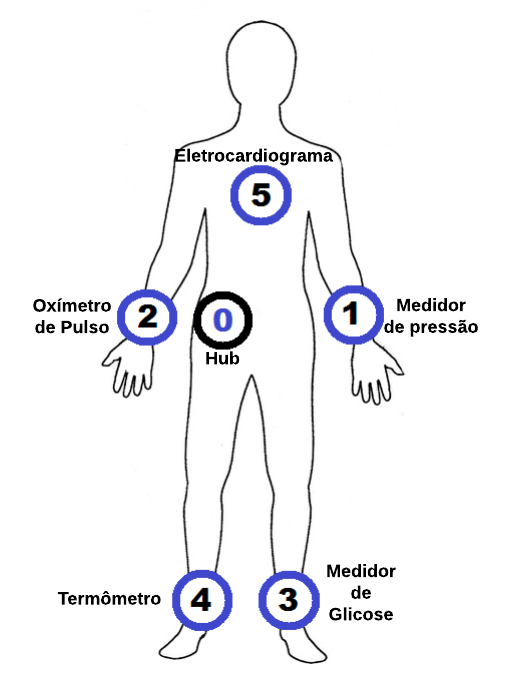
\includegraphics[scale=0.29]{figures/corpoSensoresNomes.png}}
%\caption{The simulated network topology.}
%\label{fig:wbantopology}
%\end{figure}

\begin{figure}[htbp]
\centering
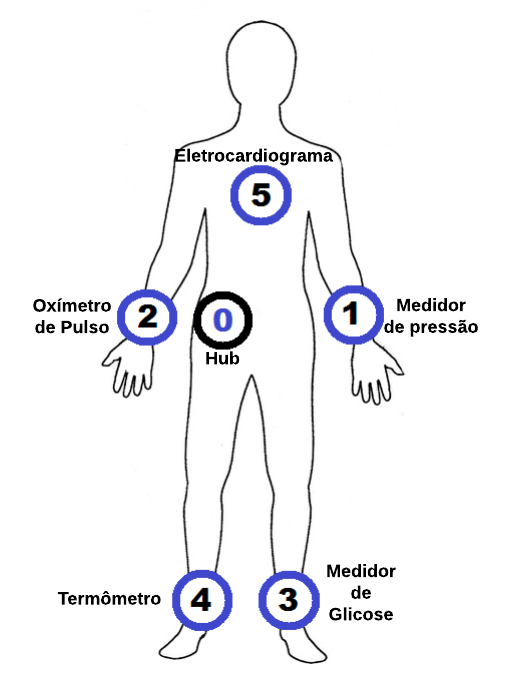
\includegraphics[width=.3\textwidth]{figures/corpoSensoresNomes.png}
\caption{Topologia da rede utilizada nas simulações.}
\label{fig:wbantopology} 
\end{figure}

%In this work, we simulate three scenarios. In the first scenario, called \textbf{unconfirmed mode}, agents send measurements with no confirmation by the manager. In the second scenario, called \textbf{retransmission mode}, agents expect an ACK from the manager during three seconds and in case it is not received, the packet is retransmitted up to three times, after that, a new association is made. The third and last one, \textbf{confirmed mode}, agents wait for three seconds the ACK from the manager. If an ACK is not received, the agent has to try to establish a new association to finalize the transmission of the measurement packets. Table \ref{3modes} summarizes the three mentioned modes.
%Neste trabalho, nós simulamos três cenários diferentes. No primeiro cenário, chamado de \textbf{unconfirmed mode}, os agentes enviam leituras sem esperar nenhuma confirmação do gerente. No segundo cenário, \textbf{retransmission mode}, onde é aplicado nossa proposta, os agentes esperam por confirmação por cada pacote de leitura enviada e, fazem a retransmissão dos pacotes caso uma confirmação não seja recebida. No terceiro e último cenário, \textbf{confirmed mode}, os agentes esperam uma confirmação durante três segundos, se um ACK não for recebido neste período, uma nova associação é estabelecida para finalizar a transmissão dos pacotes.  A tabela \ref{3modes} resumo os três cenários apresentados.
O cenário de simulação utilizado foi definido da seguinte forma: utilizando o modo de retransmissão, os agentes esperam por uma confirmação dos pacotes enviados, por um tempo definido pelo usuário no parâmetro \textit{timeOutToRetransmitPacket}, se nenhuma confirmação é recebida, é feita a retransmissão desse pacote por até \textit{maxNumOfRetransmition} vezes, também definido pelo usuário. Se o valor \textit{maxNumOfRetransmition} de retransmissões for atingido, uma nova associação é estabelecida. Foram usados cinco valores diferentes para \textit{timeOutToRetransmitPacket}, $200$, $400$, $600$, $800$ e $1000$ milissegundos. Para \textit{maxNumOfRetransmition} utilizamos $6$, $7$, $8$, $9$ e $10$, totalizando 25 cenários diferentes.

%The MAC layer used is the IEEE 802.15.6 (WBAN) \cite{b5} with path loss map and temporal model for wireless channel supplied by Castalia, and we use a 1024 Kbps physical data rate. The radio used meets with the IEEE 802.15.6 radio proposal \cite{b5} with $-15$dBm as transmission power.
%VINICIUS - Faltou colocar as referências para o padrão do MAC e dizer quantas retransmissões são usadas no retransmission mode% R: Feito
Foi utilizada a camada MAC definida pelo padrão IEEE 802.15.6 (WBAN) \cite{b5} com mapa de perda de sinal e modelo temporal para o canal sem fio fornecidos pelo simulador Castalia. A taxa de transmissão na camada física de $1024$ Kbps e o rádio utilizado, se enquadram na proposta do padrão IEEE 802.15.6, trabalhando com $-15$dBm para transmissão.

%\begin{table}[htbp]
%\caption{Modos de operação implementados na aplicação proposta}
%\begin{center}
%\begin{tabular}{lllll}
%\cline{2-4}
% & \multicolumn{1}{c}{\textbf{\begin{tabular}[c]{@{}c@{}}Modo\\ sem confirmação\end{tabular}}}                      & \multicolumn{1}{c}{\textbf{\begin{tabular}[c]{@{}c@{}}Modo com\\ retransmissão\end{tabular}}}                                      & \multicolumn{1}{c}{\textbf{\begin{tabular}[c]{@{}c@{}}Modo com\\ confirmação\end{tabular}}}                                         &  \\ \cline{2-4}
%& \begin{tabular}[c]{@{}l@{}}As leituras \\ são transmitidas\\ sem confirmação \\ do gerente.\end{tabular} & \begin{tabular}[c]{@{}l@{}}As leituras \\ são retransmitidas\\ se um ACK não\\ for recebido\\  do gerente.\end{tabular} & \begin{tabular}[c]{@{}l@{}}Se um ACK não\\ for recebido, tente\\ uma nova associação\\ para continuar a transmissão \\das leituras.\end{tabular} &  \\ \cline{2-4}
%\end{tabular}
%\label{3modes}
%\end{center}
%\end{table}

%The configuration of the nodes is set as follows: the total simulation time is 100 seconds. Node 0 uses the \textit{Manager} application and is the hub. The blood pressure and the pulse oximeter transmit one measurement per second, totalizing 100 measurements to be sent in our simulation. The thermometer sends one read every 2 seconds, then, 50 measurements should be sent. The glucose meter transmits one measurement every 25 seconds, that is, 4 measurements in 100 seconds. In this work, we assume the basic ECG as a device that receives signals of all electrodes deployed in the body, and transmit these signals to the manager. It will transmit 80 millivolt samples per 0.8 seconds, which gives 125 measurement packets in 100 seconds of simulation.
As configurações dos nós são definidas da seguinte forma: O nó zero é o hub e usa a aplicação \textit{Manager}. Os demais nós são agentes e usam a aplicação \textit{Agent}. Ambas as aplicações foram desenvolvidas por este trabalho. O medidor de pressão e o oxímetro de pulso transmitem uma leitura por segundo para o gerente, totalizando $100$ leituras durante toda a simulação. O termômetro envia uma leitura a cada 2 segundos, assim, 50 leituras devem ser enviadas durante a simulação. O medidor de glicose transmite apenas uma leitura a cada 25 segundos, totalizando no final da simulação 4 leituras a serem enviadas. Neste trabalho, é assumido que o ECG é um dispositivo que recebe os sinais de todos os eletrodos que estiverem implantados no corpo e envia os sinais para o gerente. Este ECG transmitirá $80$ leituras por pacote a cada $0.8$ segundos, o que no final totaliza 125 leituras. Essas $80$ amostras equivalem a $0.8$ segundos de dados retirados da base de dados \cite{b2}.

\subsection{Análise dos resultados}

%All the results that will be presented is already implemented in the proposed application and everyone can feel free to customize it. 
%The results available in the application are the total control packets exchanged per node, the measurements packets received by the manager per node, the measurements packets sent by each node, and the total of associations made per agent. 

% The first result discussed is the total of successfully measurements delivered to the manager. As described in \cite{b1}, when an agent is working on confirmed mode, it  should send a measurement packet and wait for the ACK during three seconds. 
Analisar a quantidade de leituras que foram entregues com sucesso no gerente é fundamental para averiguar a eficiência do método de transmissão. Na Figura \ref{fig:leiturasEntregues}, é exibida a quantidade de leituras entregues por cada um dos dispositivos, em cada um dos vinte e cinco cenários analisados, utilizando o mecanismo proposto e, na Figura \ref{fig:leiturasEntregues2modes} é possível ver o desempenho dos três modos onde, foi utilizado o cenário \textit{maxNumOfRetransmition} = 6 e \textit{timeOutToRetransmitPacket} = 200ms para o modo de retransmissão. 

\begin{figure}[htbp]
\centering
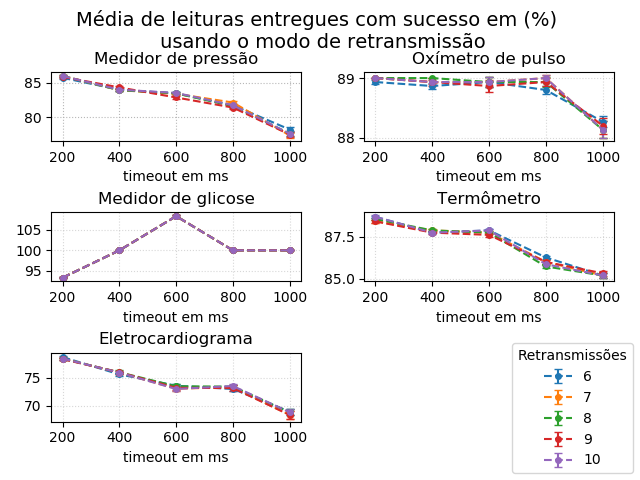
\includegraphics[width=.7\textwidth]{figures/mediaDeLeiturasEntregues.png}
\caption{O eixo $y$ representa a percentagem de leituras entregues e o eixo $x$ os valores de  \textit{timeOutToRetransmitPacket}. Cada linha do gráfico representa um valor de \textit{maxNumOfRetransmition}.}
\label{fig:leiturasEntregues} 
\end{figure}

É possível observar na Figura \ref{fig:leiturasEntregues} que a maioria dos pacotes são transmitidos quando o menor \textit{timeout} de $200$ milissegundos é utilizado. Este resultado é esperado, pois a simulação possui tempo finito e, quanto maior o \textit{timeout}, menos tempo para enviar leituras o dispositivo possui. Por outro lado, a qualidade do enlace sem fio e a quantidade de leituras transmitidas influenciam diretamente neste resultado. Enquanto o medidor de glicose envia apenas quatro leituras em $100s$, o ECG - que possui o pior link entre todos os dispositivos, tem que enviar 125 em $100s$ apenas.

\begin{figure}[H]
\centering
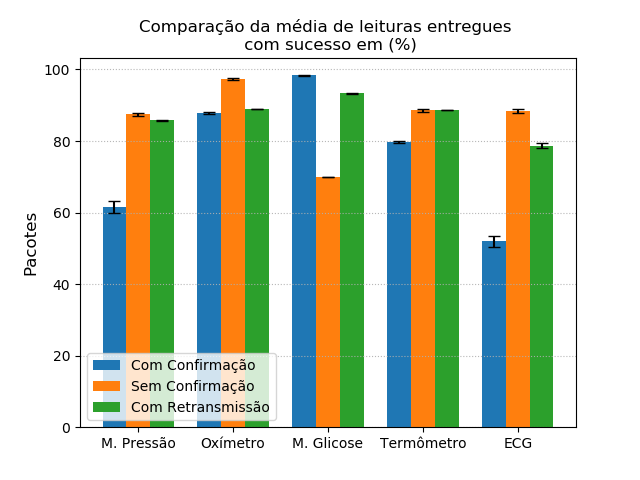
\includegraphics[width=.6\textwidth]{figures/mediaDeLeiturasEntregues2modes.png}
\caption{O eixo $y$ representa a percentagem de leituras entregues e o eixo $x$ os agentes. Cada linha do gráfico representa um modo de operação.}
\label{fig:leiturasEntregues2modes}
\end{figure}

% We can see in Fig.~\ref{fig:measurementreceivedpernode} the lack of adaption of the confirmed mode to the scenario, due to lost ACKs, timeouts and disassociation/reassociation processes. The retransmission mode improved the results by reducing the wait time of an association handshake, and retransmitting the messages sooner. The unconfirmed mode delivered almost all packets, although it provides no reliability.
%VINICIUS - Poderia quantificar a melhoria do retransmission em relação ao confirmed%

No modo de operação com confirmação, apenas o oxímetro e medidor de glicose entregaram mais de $85\%$ das leituras. Devido o modo de operação sem confirmação não utilizar nenhum mecanismo de entrega confiável e nenhum \textit{timeout} durante a transmissão, obteve um bom desempenho em quase todos os dispositivos.

% The overhead of control packets exchanged between a node and the manager is crucial in this scenario, as in the case of a new association due to a non-received ACK. The association procedure involves a maximum of four packets for a new node, and a minimum of two packets, when the agent's attributes are previously known.

% The total average of control packets exchanged between each node and the manager per operation mode is depicted in Fig.~\ref{fig:controlpacketsexchanged}. Notice that our retransmission mode saves about $21.5\%$ of control packets when compared to the confirmed mode. The unconfirmed mode as expected is the one that transmits less control packets.
Podemos observar que existe um \textit{trade-off} quando $200$ milissegundos é utilizado como \textit{timeout}. Na Figura \ref{fig:retransmicoes}, é possível ver que o maior número de retransmissões ocorreu quando $200$ milissegundos foi utilizado. Isso acontece em razão do gerente não enviar uma resposta dentro do tempo limite, fazendo com que os agentes reenviem o pacote por falta de ACK. O gráfico apresentado possui apenas valores do cenário onde \textit{maxNumOfRetransmition} é igual a $6$, pois, a partir da sétima retransmissão, os valores tendem a ficar próximos de zero, como pode ser visto na Figura \ref{fig:retransmicoes}.

\begin{figure}[htbp]
\centering
\begin{minipage}{.5\textwidth}
\centering
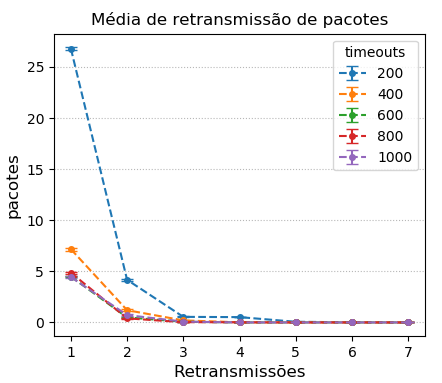
\includegraphics[width=.9\textwidth]{figures/retransmicoes.png}
\caption{Retransmissões de pacotes utilizando \textit{timeouts} diferentes.}
\label{fig:retransmicoes}
\end{minipage}%
\centering
\begin{minipage}{.5\textwidth}
\centering
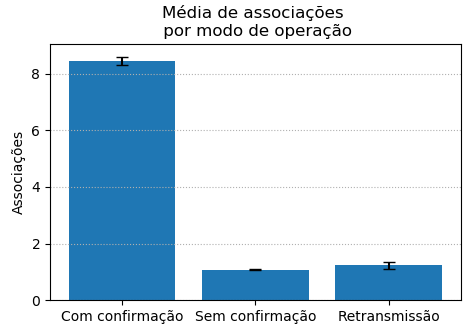
\includegraphics[width=.9\textwidth]{figures/associacoes.png}
\caption{Média de associações feitas por agente, para o cenário com \textit{maxNumOfRetransmition} = $6$ e  \textit{timeOutToRetransmitPacket} = $600$ ms.}
\label{fig:associacoes} 
\end{minipage}
\end{figure}

Pode-se ver a redução no número de associações feitas por cada agente, entre o modo de operação com confirmação e o modo proposto no artigo na Figura \ref{fig:associacoes}. Em média, no modo de retransmissão, cada agente precisou estabelecer menos de duas associações para concluir a transmissão de leituras, enquanto o modo com confirmação usou em média mais de oito associações em cada transmissão. Isso representa uma economia de até 32 pacotes de controles, e vários \textit{timeouts} evitados. 

% \begin{figure}[htbp]
% \centering

% \end{figure}

% The number of associations made per node is extremely high with the confirmed mode, since it tries a new association after every packet lost. Fig.~\ref{fig:associationnumber} shows the average number of associations that each node made in the three operation modes. As expected, the confirmed mode has the highest average of association attempts, while the unconfirmed mode made just one association. The retransmission mode tries a new association after all the attempts to resend a message fail, or if the agent receives an abort message from the manager. This is the reason for the low average of associations in this mode.   
Na Figura \ref{fig:latencia}, nota-se que a maioria dos pacotes possuem uma latência média de $30$ milissegundos. O tempo é calculado desde a criação do pacote, na camada de aplicação do agente, até o recebimento do mesmo na camada de aplicação do gerente. Os valores mostrados são referentes ao cenário onde \textit{maxNumOfRetransmition} é igual a $6$ e  \textit{timeOutToRetransmitPacket} é igual a $200$ ms.

\begin{figure}[htbp]
\centering
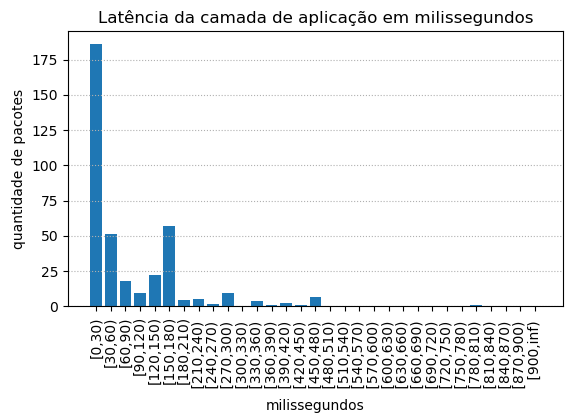
\includegraphics[width=.6\textwidth]{figures/latencia.png}
\caption{Latência média da camada de aplicação dos agentes, para o cenário com \textit{maxNumOfRetransmition} = $6$ e  \textit{timeOutToRetransmitPacket} = $200$ ms.}
\label{fig:latencia} 
\end{figure}

Como visto nos resultados apresentados, o modo sem confirmação obteve uma das melhores performances, pois não possui nenhum tipo de mecanismo de entrega confiável e nem confirmação de entrega. O modo de retransmissão, alcançou um bom desempenho mesmo perdendo às vezes para o modo sem confirmação. Este modo entregou cerca de $15\%$ mais pacotes de leituras e economizou $20.5\%$ pacotes de controle, quando comparado ao modo com confirmação. Este último, infelizmente, demanda muito tempo e associações, o que resulta num \textit{delay} alto e poucos pacotes entregues com sucesso.




